% Guia: practicas de codificacion, control de versiones, CI/CD y ambientes
% de despliegue.

Thary es un sistema que se desarrollo mediante el uso de las siguientes tecnologias: Python, Flask como framework, librerías como scikit-learn, Pandas, y XGBoost. 

A la hora de ejecutar el sistema en Flask, se tiene que ejecutar el comando \texttt{run.py} en un entorno virtual (\textit{venv}), todas las dependencias necesarias para la correcta ejecución del proyecto se encuentran resumidas en el archivo \texttt{requirements.txt} para su fácil instalación. 

Por su parte, el control de versiones del sistema se llevó a cabo mediante una seria de commits en GitHub en el que se documentaron los cambios más significativos del sistema durante todo el tiempo de desarrollo. 

\subsubsection{Construcción}

La principal práctica de codificación que se siguio durante el desarrollo e implementación del sistema Thary es la separación de responsabilidades, práctica la cual se vio reflejada en la organización de archivos y carpetas del proyecto:

\begin{verbatim}
sistema_prediccion_inventario/
├── app/
│   ├── routes/                 
│   │   ├── auth.py            
│   │   └── main.py            
│   ├── services/                
│   │   ├── auth.py              
│   │   ├── db.py                
│   │   ├── pedidos.py            #   Registro de pedidos confirmados
│   │   ├── actividad.py          #   Acciones de usuario
│   │   └── prediccion/           # pipeline
│   │       ├── carga_datos.py     #   1. Carga y limpieza
│   │       ├── segmentacion.py    #   2. Segmentacion ABC/variabilidad
│   │       ├── features.py        #   3. Construccion de variables
│   │       ├── modelos.py         #   4. Entrenamiento y seleccion
│   │       ├── regresion_lineal.py#   4.1. Modelo de Regresion Lineal
│   │       ├── validacion.py      #   5. Validacion cruzada temporal
│   │       ├── pronostico_futuro.py# 6. Pronostico recursivo
│   │       ├── reposicion.py      #   7. Puntos de reorden y EOQ
│   │       ├── graficas.py        #   8. Generacion de graficos
│   │       └── exportacion.py     #   9. Exportacion de resultados
│   └── templates/                
└── tests/                        # pytest
    ├── test_carga_datos.py
    ├── test_modelos.py
    └── test_reposicion.py
\end{verbatim}

Como se puede observar, la organización se divide en tres capas: \texttt{routes/} con el control del sistema, \texttt{services/} con la lógica de negocio y, dentro de esta última, \texttt{prediccion/}. Es en esa última capa, en la cual cada una de las 9 etapas del pipeline se encuentran alojadas en nueve módulos independientes: carga de datos, segmentación, construcción de variables, modelos, validación, pronóstico, reposición, gráficas y exportación. La principal ventaja de esta organización, es que permite que se pueda modificar una etapa específica del flujo sin afectar directamente a las demas partes, además de facilitar el mantenimiento y un entendimiento más fácil del código.

Como complemento a esta organización, se incorporaron pruebas automatizadas escritas con \textit{pytest}, las cuales fueron agrupadas en tres archivos dentro de la carpeta \texttt{tests/}:

\begin{itemize}
    \item \texttt{test\_carga\_datos.py}, en este archivo se verifican los mensajes de error ante archivos invalidos y el reconocimiento de columnas heterogeneas
    \item \texttt{test\_modelos.py}, en el que se verifica la lógica de selección del modelo campeón por producto
    \item y por último,\texttt{test\_reposicion.py}, en donde se verifican los calculos de stock de seguridad, punto de reorden y EOQ
\end{itemize}

(Los resultados obtenidos al ejecutar esta suite de pruebas se presentan en el Capítulo 4.)

\subsubsection{Integración}

Las rutas de la aplicación se organizan en el archivo \texttt{app/\_\_init\_\_.py}, mediante el mecanismo de Blueprints de Flask, el cual permite que se pueda agrupar un conjunto de vistas en un módulo independiente y registrarlo en la aplicación principal. Thary cuenta con dos blueprints: \texttt{main\_bp} (dashboard, inventario, presupuesto, pedidos y panel técnico) y \texttt{auth\_bp} (inicio de sesión, registro y gestión de usuarios), que se registran de la siguiente manera:

\Needspace{4\baselineskip}
\captionof{listing}{Registro de los blueprints \texttt{main\_bp} y \texttt{auth\_bp} en la aplicación Flask.}\label{lst:registro_blueprints}
\begin{minted}{python}
app.register_blueprint(main_bp)
app.register_blueprint(auth_bp)
\end{minted}

Esta organización permite que cada blueprint se desarrolle y se pruebe de forma independiente, y que agregar un nuevo conjunto de rutas al sistema no implique tener que modificar el código de los blueprints que ya existen.

Por otra parte, para integrar correctamente el modelo de predicción con la aplicación web, en el archivo \texttt{services/sistema\_prediccion.py} se incluyó una función de entrada, \texttt{ejecutar\_sistema()}, la cual se encarga de orquestar secuencialmente las nueve etapas del pipeline y devolver un resultado. Esta decisión de integración se tomó tomando en cuenta la separación de capas ya establecida para todo el proyecto. En este caso, la capa de servicios de dominio se mantiene independiente de la de presentacion.

\Needspace{10\baselineskip}
\captionof{listing}{Función \texttt{ejecutar\_sistema}, que orquesta las nueve etapas del pipeline.}\label{lst:ejecutar_sistema}
\begin{minted}{python}
def ejecutar_sistema(
    ruta_archivo, carpeta_resultados=None, presupuesto_capital_trabajo=None, horizonte_meses=None
):
    # 1. Carga, limpieza y agregacion mensual 
    df = cargar_y_limpiar(ruta_archivo)
    df_mensual = agregar_mensual(df)

    # 2. Segmentacion de productos
    producto_comportamiento = calcular_comportamiento_producto(df, df_mensual)

    # 3. Feature engineering
    df_mensual, df_model, feature_cols = construir_features(df_mensual, producto_comportamiento)

    # 4. Modelos
    modelo_lr, pred_lr, features_lr = entrenar_regresion_lineal(X_train, y_train, X_test, feature_cols)
    model, pred_xgb = entrenar_xgboost(X_train, y_train_log, X_test)
    pred_baseline_3 = prediccion_baseline_movil(test_df)

    # 5. Validacion cruzada temporal
    detalle_validacion_cruzada, resumen_validacion_cruzada = validacion_cruzada_temporal(df_model, feature_cols)

    # 6. Pronostico recursivo de los proximos N meses
    pronostico_futuro_df, ... = generar_pronostico_futuro(...)

    # 7. Puntos de reorden y EOQ
    reorder_df, ... = calcular_tabla_reorden(...)

    # 8. Graficas y exportacion de artefactos
    ...

    return {...}
\end{minted}

Otro punto de integración relevante es que Thary tiene dos maneras de almacenar la información: la base de datos relacional (MySQL), para datos que sean estructurados como números o textos cortos y el sistema de archivos para archivos que por su naturaleza no se podría poner en una tabla, en el caso de Thary, estos archivos serían el archivo del modelo XGBoost ya entrenado, y las imágenes de las gráficas. Cada vez que se procesa un CSV, en MySQL se agrega una fila nueva, nunca se borra nada, pero los archivos, es decir, las gráficas, modelo entrenado, etc, van siempre a la misma carpeta de la empresa a la que pertenezcan, y cada vez que se procesa un nuevo archivo, se sobrescriben los anteriores. Así que, si se hace una serie de corridas, en MySQL habrá varias filas completas, pero en la carpeta, solo existirán los archivos de la última corrida. 

\texttt{app/routes/main.py}:
\Needspace{8\baselineskip}
\captionof{listing}{Función \texttt{carpeta\_resultados}, que define la carpeta de resultados de cada empresa.}\label{lst:carpeta_resultados}
\begin{minted}{python}
def carpeta_resultados(empresa_id):
    """Carpeta donde ejecutar_sistema escribe el pronostico, los
    graficos y demas archivos de resultado de una empresa puntual."""
    ruta = os.path.join(current_app.config["RESULTADOS_FOLDER_BASE"], empresa_id)
    os.makedirs(ruta, exist_ok=True)
    return ruta
\end{minted}

La ruta de la carpeta depende del id de la empresa (\texttt{empresa\_id}), y no del id de la corrida (\texttt{corrida\_id}), por lo que, la carpeta siempre es la misma para una misma empresa, sin importar cuantas veces se haya procesado un archivo. 

Por otra parte, tal como se explicó en capítulos anteriores, se definió un control de acceso basado en roles, esto con el objetivo de poder diferenciar a que funcionalidades debe tener acceso un usuario dependiendo de su rol. El administrador (\texttt{admin}) debe ser el único usuario que cuente con todos los privilegios de acceso a la información sensible de la organización, mientras que para otros usuarios con menor rango, (\texttt{empleado}), convendría restringir este acceso completo a solo aquellas funcionalidades menos invasivas que sean necesarias para el desempeño de su trabajo, como todas aquellas que describen el análisis de los datos y la lista de pedidos: 

\texttt{app/services/auth.py}:
\Needspace{10\baselineskip}
\captionof{listing}{Decorador \texttt{admin\_required}, que restringe el acceso de una ruta al perfil administrador.}\label{lst:admin_required}
\begin{minted}{python}
def admin_required(vista):
    @wraps(vista)
    def envoltura(*args, **kwargs):
        if "username" not in session:
            flash("Inicia sesión para continuar.")
            return redirect(url_for("auth.login"))
        if session.get("rol") != "admin":
            flash("Esa sección es solo para el administrador.")
            return redirect(url_for("main.dashboard"))
        return vista(*args, **kwargs)
    return envoltura
\end{minted}

\paragraph{Integración continua (CI)}

El proyecto utilizó GitHub Actions para la automatización de pruebas unitarias (\texttt{.github/workflows/tests.yml}). Este se ejecuta automaticamente cada vez que se haga un \textit{push} o \textit{pull request} en el repositorio. El archivo cuenta con una configuración que permite instalar tanto Python como todas las dependencias necesarias, y ejecuta las pruebas unitarias con \texttt{pytest}:  

\Needspace{10\baselineskip}
\captionof{listing}{Flujo de trabajo de GitHub Actions para ejecutar las pruebas automatizadas (\texttt{tests.yml}).}\label{lst:github_actions}
\begin{minted}{yaml}
name: Tests

on:
  push:
  pull_request:

jobs:
  tests:
    runs-on: ubuntu-latest
    steps:
      - uses: actions/checkout@v4

      - uses: actions/setup-python@v5
        with:
          python-version: "3.12"
          cache: "pip"

      - run: pip install -r requirements.txt

      - run: pytest tests/ -q
\end{minted}

El flujo solo cubre la parte de CI (Integración Continua), en cuanto a CD (Despliegue Continuo), se decidió hacerlo de manera manual, principalmente porque 
al ser un proyecto desarrollado por una sola persona, es decir, sin múltiples entornos ni
un equipo que dependa de constantes despliegues, el beneficio de
un pipeline de CD completo es menor frente a la complejidad adicional que
implicaría configurarlo.

\subsubsection{Despliegue}

El despliegue del sistema Thary (además del entorno de desarrollo local), se encuentra en la nube mediante la plataforma Railway. 

\begin{figure}[H]
    \centering
    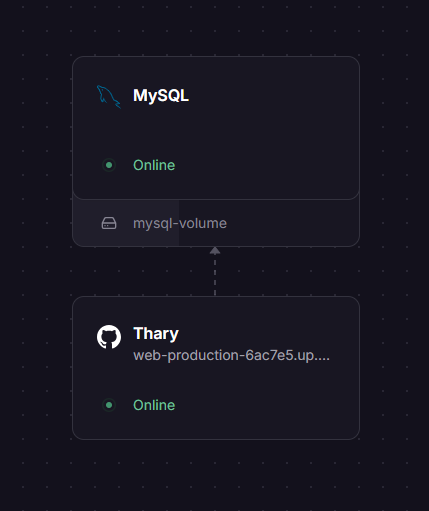
\includegraphics[width=0.6\textwidth]{templatefigures/railway_servicios}
    \caption{Servicios desplegados en Railway: aplicación web (Thary) y base de datos MySQL.}
    \label{fig:railway_servicios}
\end{figure}

Como se ve en la figura, Thary y la base de datos, se encuentran corriendo en Railway como servicios independientes, los cuales se comunican entre si para compartir información y funcionalidades.

La aplicación se ejecuta mediante un servidor WSGI de producción (Gunicorn), configurado a través del archivo \texttt{Procfile}:

\Needspace{3\baselineskip}
\captionof{listing}{Contenido del archivo \texttt{Procfile} para el servidor Gunicorn.}\label{lst:procfile}
\begin{minted}{text}
web: gunicorn run:app --bind 0.0.0.0:$PORT --workers 2 --timeout 120
\end{minted}

\begin{figure}[H]
    \centering
    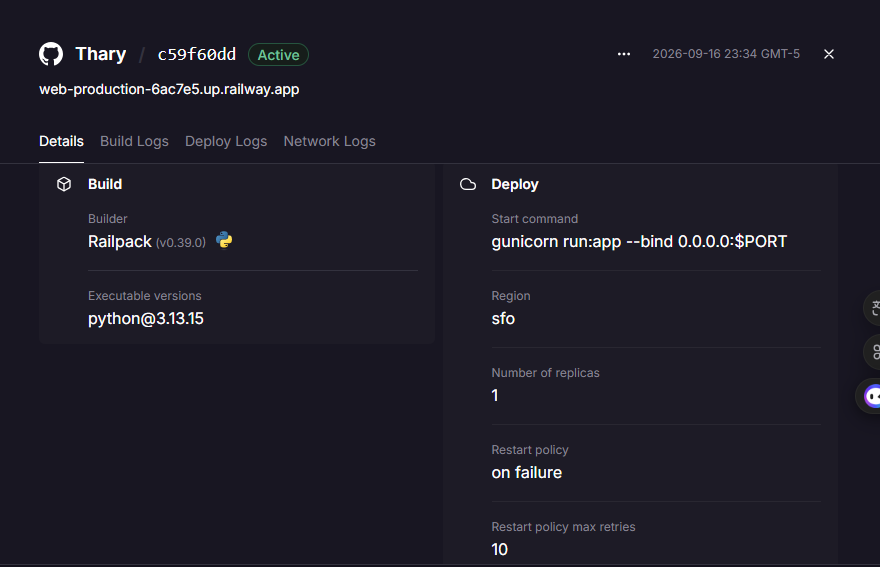
\includegraphics[width=0.85\textwidth]{templatefigures/railway_deploy_details}
    \caption{Detalles de construcción y despliegue del servicio Thary en Railway.}
    \label{fig:railway_deploy_details}
\end{figure}

Railway detecta y se encarga de ejecutar este comando \textit{start command} cuando se realiza un despliegue. Automáticamente identifica la versión de python con la que se está trabajando, en este caso, \texttt{.python-version} (3.13).  El proyecto fija todas sus dependencias en \texttt{requirements.txt}, incluyendo las versiones exactas de las librerías de predicción (pandas, scikit-learn, XGBoost, statsmodels) y las necesarias para la conexión a la base de datos (\texttt{SQLAlchemy}, \texttt{PyMySQL}) y el servidor de producción (\texttt{gunicorn}).

En cuanto a la persistencia de los datos, esta se manejó mediante MySQL. La configuración de conexión a la base de datos solo se obtiene de las variables de entorno, tal como se detalló en la Sección \ref{sec:modelo_datos} (función \texttt{\_config()}).

% \begin{minted}{python}
% def _config():
%     return {
%         "host": os.environ.get("DB_HOST", "127.0.0.1"),
%         "port": os.environ.get("DB_PORT", "3307"),
%         "user": os.environ.get("DB_USER", "thary_app"),
%         "password": os.environ.get("DB_PASSWORD", ""),
%         "database": os.environ.get("DB_NAME", "sistema_inventario"),
%     }
% \end{minted}

\begin{figure}[H]
    \centering
    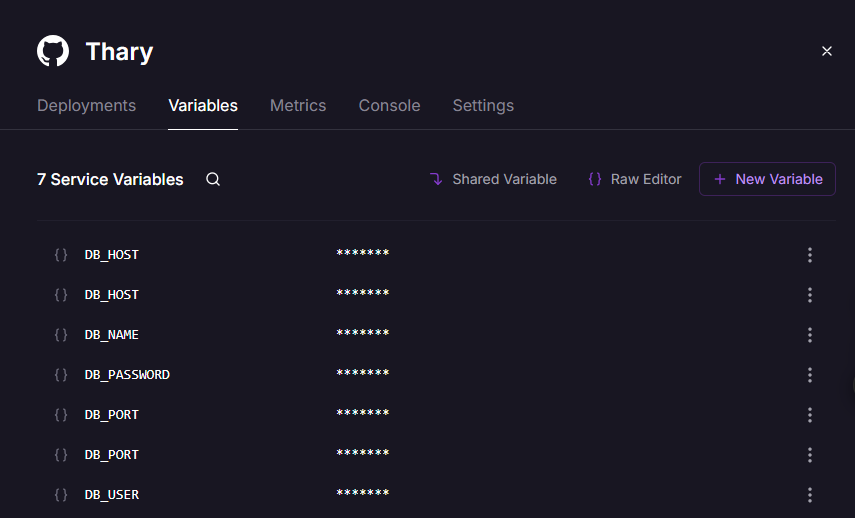
\includegraphics[width=0.7\textwidth]{templatefigures/railway_variables}
    \caption{Variables de entorno del servicio Thary en Railway, con los valores ocultos.}
    \label{fig:railway_variables}
\end{figure}

Las credenciales se configuran en el panel de Railway como variables de entorno del servicio,  nunca visibles en el repositorio de código. 

\begin{figure}[H]
    \centering
    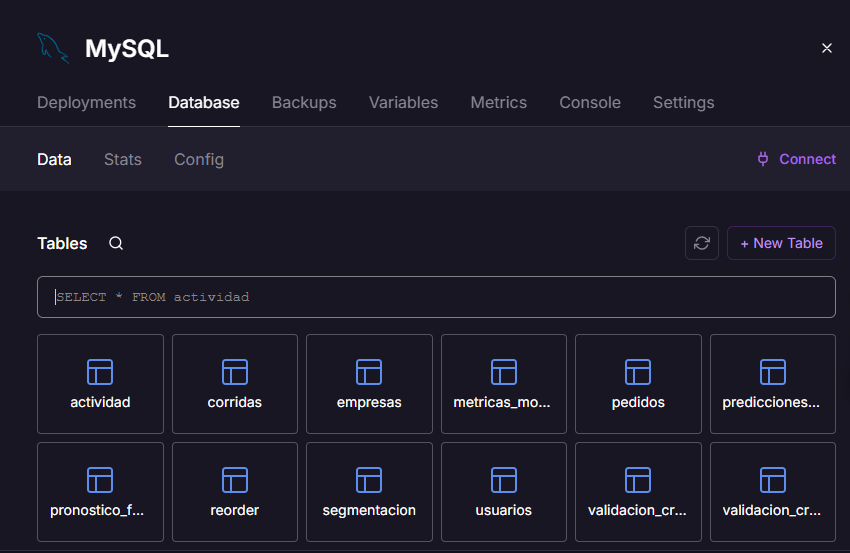
\includegraphics[width=0.75\textwidth]{templatefigures/railway_mysql_tablas}
    \caption{Tablas del esquema relacional de Thary en el entorno de producción, vistas desde el explorador de datos de Railway.}
    \label{fig:railway_mysql_tablas}
\end{figure}

La Fig. \ref{fig:railway_mysql_tablas} muestra que el mismo esquema de 12 tablas que se tiene localmente, también existe en el entorno desplegado de Railway.

El servicio de Thary no cuenta con un volumen configurado, esto puede verse en el panel de administración en el que no se ve la pestaña de "volúmenes". Esto quiere decir que los archivos que están en el servicio son efímeros, es decir, cada vez que se redespliegue el servicio, como por ejemplo, por una actualización del código o un reinicio del servicio, se crea un nuevo contenedor, por lo que se pierden por completo los archivos generados por el sistema en las corridas anteriores del pipeline. Esto se reconoce como una limitación del entorno de producción. 

\begin{figure}[H]
    \centering
    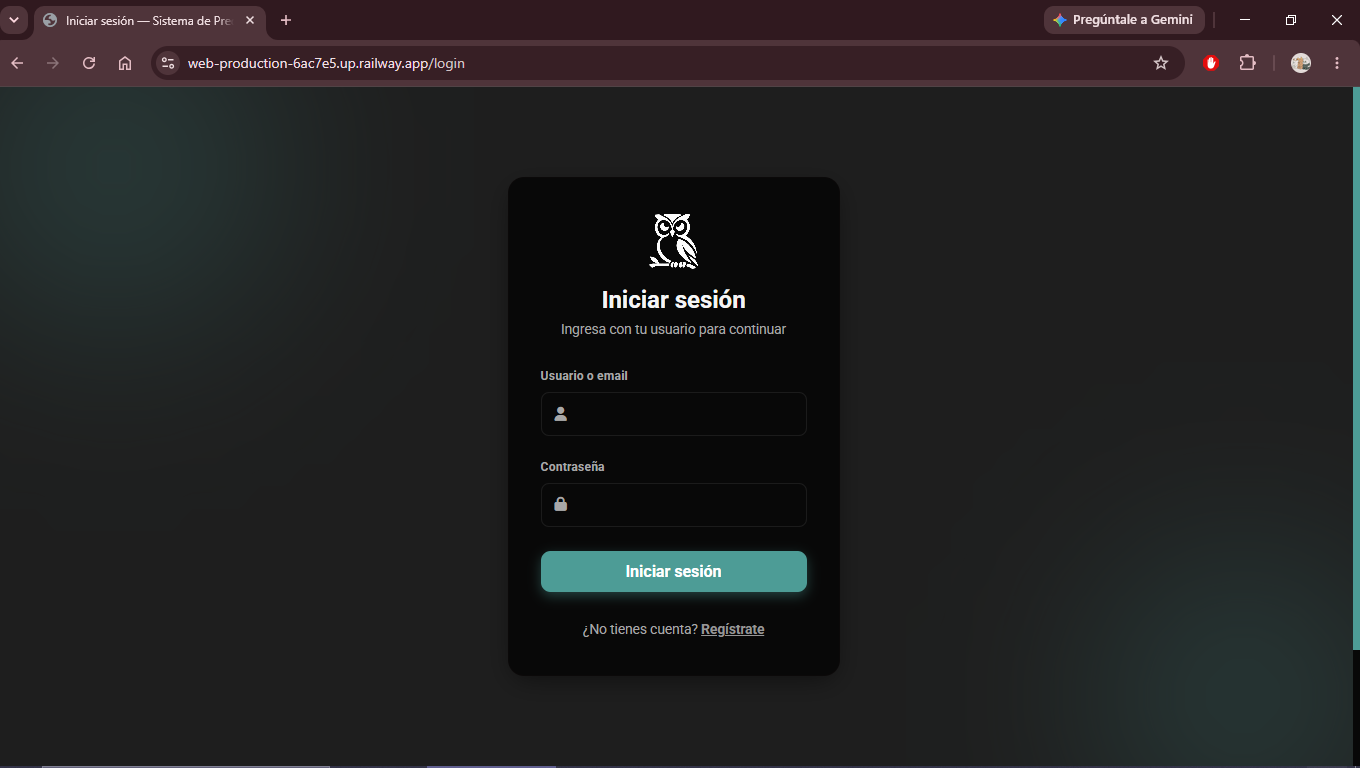
\includegraphics[width=0.75\textwidth]{templatefigures/thary_login_produccion}
    \caption{Pantalla de inicio de sesión de Thary, accedida desde su URL pública en Railway.}
    \label{fig:thary_login_produccion}
\end{figure}

Finalmente, la figura muestra la aplicación funcionando correctamente en el entorno de producción a través de de la URL pública asignada por Railway.
